\newpage
\part{Feature lifespan and design assessment}\label{part:lf}

\section{Introduction to lifespan and design mapping} \label{sec:lfintro}
Survival thresholds applied to a sequence of habitat enhancement features, can be spatially compared with hydraulic and sediment data as a result of 2D numerical modeling. Modeled discharges can be associated with flood return periods that determine feature lifespans. The resulting lifespan maps indicate the temporal stability of particular stream design features and techniques. Areas with particularly low or high lifespans help planners optimize the design and positioning of features. Moreover, discharges related to specific flood-return periods enable probabilistic estimates of the longevity of particular features. Following these procedures described by \citet{schwindt19a}, the \textit{LifespanDesign} module creates \texttt{raster}s, \texttt{mxd}-layouts and \texttt{pdf}-maps of the following types:
\begin{itemize}
	\item \textbf{Lifespan maps} qualitatively indicate areas where features make sense and the associated feature lifetime estimate in years.
	\item \textbf{Design maps} indicate dimensional requirements for achieving the success of a feature, e.g., the minimum required block (grain) sizes for angular boulders (rocks) stability.
\end{itemize}

This chapter explains the usage of the \textit{LifespanDesign} module and it is structured as follows:\\
\begin{tabular}{l L{0.9\textwidth}}
\multicolumn{2}{l}{}\\
Section~~\ref{sec:lfgui}: & Quick Guide to the application of the code using GUI with descriptions of required input rasters and alternative launch options.\\
%Section~\ref{sec:output}:& Descriptions of outputs and procedures for half-automated pdf-map generation.\\
Section~~\ref{sec:par}:   & Physical explanations of relevant parameters.\\
Section~~\ref{sec:feat}:  & Explanations of hypotheses and restoration features.\\
Section~~\ref{sec:inp}:   & Detailed explanation of input file usage.\\
Section~\ref{sec:code}:  & Detailed explanations of coding conventions with descriptions of extension possibilities.\\
\multicolumn{2}{l}{}\\
\end{tabular}


\section{Quick GUIde to lifespan and design maps} \label{sec:lfgui}
\subsection{Interface and choice of features}
The introduction (Sec.~\ref{sec:gui}) explains required modifications of the module batch launcher (\texttt{LAUNCH{\myUnderscore}Windows{\myUnderscore}x64.bat}) environment.\\
Figure~\ref{fig:gui_start_lf} shows the modules GUI at start-up, which may take a couple of seconds to launch because the module creates some of its menu entries from a spreadsheet. To begin, click on the drop-down menu ``Add Features'' and select relevant features. Multiple selection is possible and will extend the ``Selected features'' list. The \textit{LifespanDesign} module enables the selection of the feature groups ``terraforming'' (framework), ``vegetation plantings'', ``other (soil) bioengineering'' and ``maintenance'' according to the descriptions in Sec.~\ref{sec:feat}. Soil bioengineering considers slope stability in the \textit{MaxLifespan} and \textit{ModifyTerrain} modules.
\begin{figure}[hbt]
	\begin{center}
	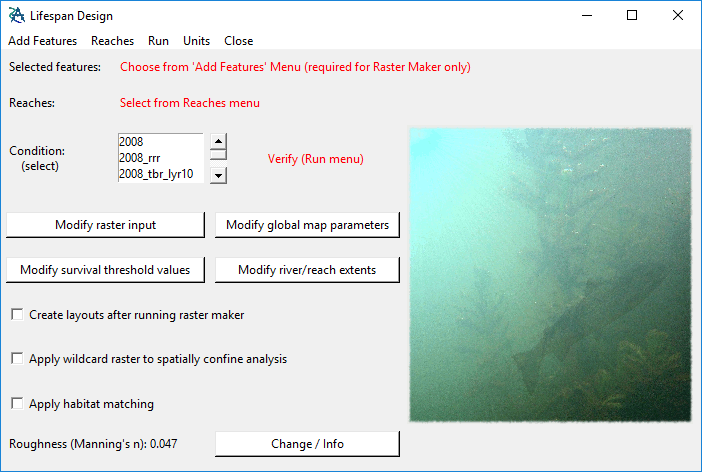
\includegraphics[width=1.0\columnwidth]{gui_start_lf.PNG} % Example image
	\caption{GUI start up window. \label{fig:gui_start_lf}}
	\end{center}
\end{figure}



\subsection{Input: Condition and preparation of rasters}\label{sec:inpras}
The names of input raster files are defined in a proper file format (\textit{.inp}), which can be changed directly from the GUI button ``Modify raster input''. The \textit{.inp} files indicates where it requires singles rasters only (\texttt{STRING}) or lists of rasters (min. two rasters, \texttt{LIST}). The maximum number of rasters is unlimited, but it is recommended to use less than ten rasters to limit the calculation duration. The lifespans related to the hydraulic rasters are defined in the \textit{.inp} file. Modifications of map extents (Sec.~\ref{sec:inpmaps}) can be made by clicking on the ``Modify map extent'' button. Sec.~\ref{sec:inpfile} provides more information on setting up the input file.


\subsection{Input: Modify threshold values} \label{sec:modthresh}
The ``Modify survival threshold values'' button opens a spreadsheet (location: \texttt{RiverArchitect/Lifespan Design/.templates/threshold{\myUnderscore}values.xlsx}), where threshold values and survival identifiers can be modified (cf. Fig.~\ref{fig:threshold_values_illu}) and modifications of the spreadsheet are intuitive. Any modification beyond the ``INPUT''-highlighted cells may corrupt the results or cause errors and program crashes. Valid changes limit to the \texttt{thresholds} sheet, while the \texttt{.templates} sheet must not be modified.\\
The ``Topographic change: inverse relevance'' threshold applies when the feature relevance refers to regions where the scour and fill rates below the specific threshold values are relevant. By default, features such as angular boulders (rocks) are relevant where the topographic change rate (scour or fill) exceeds the angular boulders (rocks) threshold value for scour rate. However, features such as grading or side cavities, are relevant where the scour or fill rates do not exceed the threshold rates because these areas are presumably disconnected from the river. Thus, ``Topographic change: inverse relevance'' is \texttt{TRUE} for the grading, side cavity, and side channel features.\\
The unit system (U.S. customary or SI metric) in the threshold values spreadsheet (Fig.~\ref{fig:threshold_values_illu}) are independent of the GUI settings but they need to be coherent with the input raster files. 

\begin{figure}[hbt]
	\begin{center}
	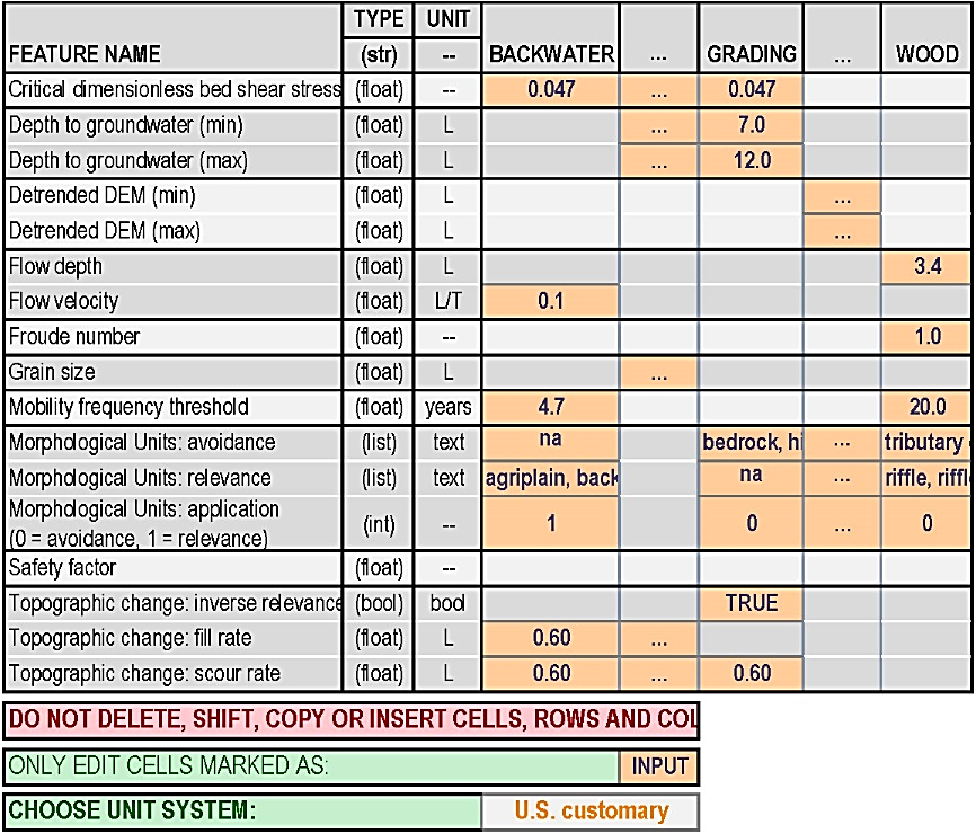
\includegraphics[width=0.78\columnwidth]{threshold_values_illu.pdf} % Example image
	\caption{Spreadsheet with threshold values and survival identifiers. \label{fig:threshold_values_illu}}
	\end{center}
\end{figure}

More on information on threshold values is provided in Sec.~\ref{sec:feat}, which discusses the identifiers and threshold value of the base case scenario (lower Yuba River in 2008).

\subsection{Input: Optional arguments}

The checkbox ``Include layout creation in raster analysis'' provides the optional automated preparation of \texttt{.mxd} files for mapping the results (see explanations in Sec.~\ref{sec:outmaps}).\\
The checkbox ``Apply wildcard raster to spatially confine analysis'' can be checked to use the \texttt{wild} raster for spatial limitation of the results. This application makes sense, e.g., if the wildcard raster contains particular land parcels, where the owner wants to foster habitat enhancement.\\
The checkbox ``Apply habitat matching'' provides the option of habitat matching to regions where the habitat suitability index is low ($<$0.4, see explanations in part \ref{part:he}).\\
Switching between unit systems (U.S. customary or SI -- metric) is possible via the drop-down menu ``Units''; please note that the unit system needs to be consistent with all input raster files.

\subsection{Run}

Once all inputs are defined, click on ``Run'' and ``Verify settings'' to ensure the consistency of the chosen settings (the window will freeze for some seconds). After successful verification, the selected options change to green font.\\

Three ``Run'' drop-down menu provides the following routines:
\begin{itemize}
\item \pythoninline{Raster Maker} prepares lifespan and design rasters in the directory \texttt{Output/Rasters/\textit{condition}/}
\item \pythoninline{Layout Maker} prepares \texttt{.mxd} layouts in the directory \texttt{Output/Mapping/\textit{condition}/Layouts};\\
by default the layout maker applies on the rasters stored in \texttt{Output/Rasters/\textit{condition}/} but it also accepts other raster input directories as an optional argument when the module is used without GUI (see Alternative Run options in Sec.~\ref{sec:lfrun}).
\item \pythoninline{Map Maker} prepares map assemblies (\texttt{pdf}s) in the directory \texttt{Output/Mapping/\textit{condition}/};\\
by default the maps are created based on the layouts stored in \texttt{Output/Mapping/\textit{condition}/} but the method also accepts other layout input directories as an optional argument when the module is used without GUI (see Alternative Run options in Sec.~\ref{sec:lfrun})
\end{itemize}

Either ``Run'' option causes a run confirmation window popping up and clicking ``OK'' calls the analysis, which will run in the background python window and it freezes the GUI windows. Running the Raster Maker takes 1 to 10 hours, depending on the feature set and habitat matching. The Layout Maker requires that rasters exist in the \texttt{Output/Rasters/\textit{condition}/} directory. After the Layout creation, manual intervention is required to run Map Maker (see explanations in Sec.~\ref{sec:outmaps}).\\

After the analysis, the GUI unfreezes and a red button will appear, which invites reading the logfiles with information, error and warning messages that occurred during the analysis.\\

Moreover, the module requires the directory \texttt{01{\myUnderscore}Conditions/\textit{condition}/} to be located in the same folder as the \texttt{.py}-files. Section~\ref{sec:input} explains the preparation of this directory.\\
The directory \texttt{Output/Mapping/.ReferenceLayouts} is essential for \pythoninline{class Mapper()}. Section~\ref{sec:inpmaps} illustrates possibilities and procedures for adapting map layouts.\\


\subsection{Alternative run options}
\label{sec:lfrun}
The three run options of the GUI call the following methods:
\begin{enumerate}
\item Raster Maker calls \pythoninline{feature_analysis.raster_maker} for the preparation of rasters in the directory \texttt{Output/Rasters/\textit{condition}/}
\item Layout Maker calls \pythoninline{feature_analysis.layout_maker} for the preparation of \texttt{.mxd} layouts in the directory \texttt{Out put/Mapping/\textit{condition}/Layouts}; this method applies on rasters stored in \texttt{Output/Rasters/\textit{con dition}/} by default but it also accepts other raster input directories as an optional argument
\item Map maker calls \pythoninline{feature_analysis.map_maker} for the preparation of maps assembled in \texttt{pdf}s in the directory \texttt{Output/Mapping/\textit{condition}/}; by default the layouts stored in \texttt{Output/Mapping/\textit{condition}/} underlie the \texttt{pdf} creation but the method also accepts other layout input directories as an optional argument\\
\textit{Please not that directories always need to be \textbf{absolute}; relative paths will result in errors.}
\end{enumerate}

The alternative run options are relevant, e.g., for the batch processing of several conditions. Moreover, the alternatives enable running the Layout Maker or Map Maker in another folder than \texttt{Output/Rasters/\textit{condition}/}. The first alternative is importing the module \textit{LifespanDesign} in the ArcGIS Python \textbf{x64} interpreter as follows:

\begin{enumerate}
	\item Prepare input in \texttt{.../01{\myUnderscore}Conditions/\textit{condition}/} folder
	\item Go to ArcGIS Python folder\\
	Example: \texttt{C:/Python27/ArcGISx64XX.X}
	\item Launch \texttt{python.exe}
	\item Enter \pythoninline{import os}
	\item Navigate to Script direction using the command \pythoninline{os.chdir("ScriptDirectory")}\\
	Example: \pythoninline{os.chdir("D:/Python/RiverArchitect/LifespanDesign/")}
	\item Import the module: \pythoninline{import feature_analysis as fa}\\
\end{enumerate}

Once the module is imported three methods are available and their use is intended in the following order:
\begin{enumerate}
	\item \pythoninline{fa.raster_maker("condition", *args)} for raster (ESRI GRID) creation
	\item \pythoninline{fa.layout_maker("condition", *args)} for layout (\texttt{.mxd}) creation
	\item \pythoninline{fa.map_maker("condition", *args)} for map (\texttt{pdf}) creation
\end{enumerate}

The following steps illustrate the application of \pythoninline{fa.raster_maker("condition", *args)} for creating rasters.
\begin{itemize}
	\item Basic execution: \pythoninline{fa.raster_maker("condition")}, for example: \pythoninline{fa.raster_maker("2008")}
	\item The code is now running (this takes two to four hours) and it will prompt its activities.
	\item Alternatively, the analysis can be limited to some features only (count 2 to 30 minutes per feature). \pythoninline{raster_maker} accepts optional arguments. which are \texttt{feature{\myUnderscore}list}, which enables the analysis of any feature listed in Sec.~\ref{sec:featoverview}, and \pythoninline{mapping}, which calls layout (\texttt{mxd}) creation. Some examples for particular applications:\\
	$\rightarrow$ Example 1: \pythoninline{fa.raster_maker("2008", ["Plantings"])} analyses plantings only.\\
	$\rightarrow$ Example 2: \pythoninline{fa.raster_maker("2008", ["Plantings", "Boulders/rocks"], True)} analyses plantings and angular boulders (rocks) only with an optional argument \pythoninline{True} that activates the creation of layouts for plantings and angular boulders (rocks).\\
	$\rightarrow$ Example 3: \pythoninline{fa.raster_maker("2008")} analyses all available features (see Sec.~\ref{sec:featoverview}).
	\item The complete list of optional arguments of \pythoninline{fa.raster_maker(...)} is as follows:\\
				\textit{Hint: Respecting the order of optional arguments is crucial to ensure proper application of the desired analysis options.}
				\begin{itemize}
				\item[\small{\texttt{args[0]}}] = \pythoninline{feature_list} as above described.
				\item[\small{\texttt{args[1]}}] = \pythoninline{mapping}, which can be \pythoninline{True} or \pythoninline{False} (default).
				\item[\small{\texttt{args[2]}}] = \pythoninline{habitat_analysis}, which can be \pythoninline{True} or \pythoninline{False} (default) for activating or deactivating habitat delineation (limitation) of restoration features to zones with low habitat suitability (\texttt{cHSI} = 0.0 to 0.4).
				\item[\small{\texttt{args[3]}}] = \pythoninline{habitat_radius} is a \pythoninline{Float} number determining in what distance to low habitat suitability zones restoration features should be applied (default = 400.0 ft or m).
				\item[\small{\texttt{args[4]}}] = \pythoninline{unit_system} is either \pythoninline{"us"} (default) or \pythoninline{"si"}.
				\item[\small{\texttt{args[5]}}] = \pythoninline{wildcard} is either \pythoninline{True} or \pythoninline{False} (default).
				\end{itemize}
\end{itemize}

The code creates a temp folder called \texttt{.cache} where it stores temp variables, databases, and rasters. Avoid accessing \texttt{.cache} while the code is running and ensure its (manual) deletion in the case that the code crashed.\\

\pythoninline{fa.layout_maker("condition", *args)} creates layout files (\texttt{.mxd}) and it can be used as follows.
\begin{itemize}
	\item With prior creation of rasters (see above Example~2):\\
	\pythoninline{fa.raster_maker("condition", ["Featurename"], True} or \pythoninline{fa.raster_maker("condition", [], True}; please note that \pythoninline{True} needs to be given at third place and the default is \pythoninline{False} (layout creation deactivated).
	\item Creating layouts only (requires that rasters exist):\\
	Option~1: \pythoninline{fa.layout_maker("condition"} uses the raster input folder \texttt{.../Output/Rasters/\textit{condition}/} or \\
	Option~2: \pythoninline{fa.layout_maker("condition", "D:/Any/absolute/path/"} uses an alternative raster input folder (must be an absolute path); ensure finishing the path with \pythoninline{"/"} or \pythoninline{"\\\\"}
\end{itemize}

\pythoninline{fa.map_maker("condition", *args)} for creating \texttt{pdf} map assemblies requires layout files \texttt{.mxd} prepared by either \pythoninline{fa.raster_maker("condition", ["Featurename"], True} or \pythoninline{fa.layout_maker("condition"}. After either method has created layout files \texttt{.mxd}, manual intervention is required because of an \texttt{arcpy} deficiency: called outside of \textit{ArcMap Desktop}, \texttt{arcpy} works as a background process that cannot actively change layer symbology. The module has an own \texttt{ServerStyle} file stored in \texttt{.../Output/Mapping/.ReferenceLayouts}, which defines the legend style. Currently \textit{ArcGIS} can apply the styles of any \texttt{.ServerStyle} to the legend only but not to layers, even though the styles are contained in the file. For more information, follow the discussion on \href{https://community.esri.com/thread/210442-how-do-i-apply-arcpymappingupdatelayer-to-a-mapdocument-in-a-background-process}{GeoNet}.\\

In the meanwhile, manual intervention is required as explained in the Output-Section~\ref{sec:output}. Also \pythoninline{fa.map_maker("condition", *args)} accepts an optional argument defining an alternative layout input path:
\begin{itemize}
	\item Option~1: \pythoninline{fa.map_maker("condition"} uses the layout input folder \texttt{.../Output/Mapping/\textit{condition}/} 
	\item Option~2: \pythoninline{fa.map_maker("condition", "D:/Any/absolute/path/"} uses an alternative layout input folder (must be an absolute path); ensure finishing the path with \pythoninline{"/"} or \pythoninline{"\\\\"}
\end{itemize}


The second alternative is running the module as standalone script (\texttt{feature{\myUnderscore}analysis.py}) from the system command line:
\begin{enumerate}
\item Launch terminal\\
	Windows: Launch \texttt{cmd}\\
	Mac OS: Launch \texttt{Terminal.app}\\
	Linux: Open terminal 
	\item On Windows: navigate to the place where \textit{ArcGIS} \texttt{python.exe} is stored:\\
	For example: \pythoninline{C:\\Python27\\ArcGISx64XX.X\\} and pay attention using \\
	\item Run \pythoninline{feature_analysis} as script:
	\begin{itemize}
		\item Windows: \pythoninline{python.exe DriveLetter:\\...\\LifespanDesign\\feature_analysis "condition" ["Feature"}\\\pythoninline{"name"]}
		\item Linux \pythoninline{python .../feature_analysis "condition" ["Featurename"]}\\
		\textit{Hint: Ensure that python calls the correct version used by arcpy.}
	\end{itemize}
	\item The code asks for a condition, which needs to be typed case-sensitive and without any apostrophes:\\
	For example: \pythoninline{Enter the condition (shape: >> XXXX, e.g., >> 2008 ) >> 2008}
\item Next, the code asks for a \pythoninline{feature_list}, which is and optional argument (simply hitting enter will work, too); the feature list must be typed as list (in brackets):\\
	For example: \pythoninline{Enter the condition (no mandatory; do not forget brackets - example:}\\
	\pythoninline{ >> ["Featurename1", "Featurename2] >> ["Sidecavity", "Bermsetback"]}
	\item The code is now running - this takes time - and it will prompt when it finished.
\end{enumerate}
Calling the module as \texttt{.py} script may cause in errors because of differences between path interpretation methods and it is limited to the creation of rasters only. Therefore, the fastest and most consistent way for using the \pythoninline{feature_analysis} module is to import it as above described.




%----------------------------------------------------------------------------------------
\subsection{Output}
\label{sec:output}
\subsubsection{Rasters}
The output rasters are either of the types lifespan (\texttt{lf{\myUnderscore}\textit{shortname}}) or design (\texttt{ds{\myUnderscore}\textit{shortname}}) and they are created in \texttt{.../Output/Rasters/\textit{condition}/}. The usage of \texttt{\textit{shortname}}s (see list in Sec.~\ref{sec:featoverview}) is necessary because \texttt{arcpy} does cannot handle rasters with names longer than 13 characters. The analysis automatically shortens too long raster names on the basis of shortnames and it creates the condition-output directory if it does not yet exist. Existing files in the \texttt{Output/Rasters/\textit{condition}/} folder are overwritten (the code enforces overwriting and tries to delete any existing content, i.e., ensure that the output folder does not contain any important files).

\subsubsection{Layouts and Maps}\label{sec:outmaps}
The module provides a half-automated routine for mapping the rasters in \texttt{pdf}s. Full automation is not possible because when \texttt{arcpy} is called outside of an \textit{ArcMap-Desktop} application, it runs as a background process, which cannot transfer the symbology from any layer or feature to another layer or feature (see above comments in Sec.~\ref{sec:lfrun}). The following workflow can be used to obtain \texttt{pdf} maps of all rasters from \texttt{Output/Rasters/\textit{condition}/}.
\begin{enumerate}
	\item Prepare layouts
	\begin{enumerate}
	\item GUI: Either check button before launching ``Run: Raster Maker'' or directly by clicking on ``Run: Layout Maker'' from the ``Run'' menu.
	\item Alternative \texttt{python} console: Either use \pythoninline{fa.raster_maker(condition, 1)} of \pythoninline{fa.layout_maker(condition)}:
	\begin{itemize}
		\item Calling the \pythoninline{raster_maker} with the optional argument ``1'', e.g., \pythoninline{fa.raster_maker("2008", 1)} calls the function \pythoninline{fa.layout_maker} based on prepared layouts for lifespan and design maps.
		\item Directly call \pythoninline{fa.layout_maker("condition")} for creating layouts only.
		\item Directly call \pythoninline{fa.layout_maker("condition"), r"D:/Alternative/Raster/Directory/"} for creating layouts from a directory that differs from \texttt{Output/Rasters/\textit{condition}/}.
	\end{itemize}
	\end{enumerate}
	\item Python now prepares layout files (\texttt{.mxd}) in the folder \texttt{Output/Mapping/\textit{condition}/Layouts/} corresponding to the raster names in \texttt{Output/Rasters/\textit{condition}/}.
	\item Open each layout file (\texttt{lf{\myUnderscore} $\ldots$.mxd} and \texttt{ds$\_ \ldots$.mxd}) in \textit{ArcMap-Desktop} and use the following procedure to apply the symbology (see illustration in Fig.~\ref{fig:make_layouts}):
	\begin{enumerate}%[label=\alph*]
		\item In the Table of Contents, double-click on the gray-scaled \texttt{temp} layer for accessing the \textit{Properties} window.
		\item Go to the \textit{Symbology} tab and click on ``Classified'' (computing histograms is required, if queried). Click on ``Import...'' button (folder symbol in the top-right corner) and select \texttt{lf{\myUnderscore}sym{\myUnderscore}ras} (for lifespan maps) or \texttt{ds{\myUnderscore}sym{\myUnderscore}ras} (for design maps).\\
		\textit{Hint: Some layouts contain on/off (``NoData+/1) values only. In these cases, ``Unique Values'' apply instead of ``Classified''.}
		\item Click OK and the gray layer should adapt its colors.
		\item Save and exit the \texttt{.mxd} file.
	\end{enumerate}
	\item Run: Map Maker
	\begin{enumerate}
	\item GUI: Click on ``Run'' and ``Run: Map Maker''.
	\item Alternative \texttt{python} console: type and run \pythoninline{fa.make_maps(condition)}, which produces a \texttt{pdf} catalog of each layout.
	\end{enumerate}
	\item Find the maps in the \texttt{Output/Rasters/\textit{condition}/Layouts/} directory.
\end{enumerate}

\begin{figure}
	\centering
	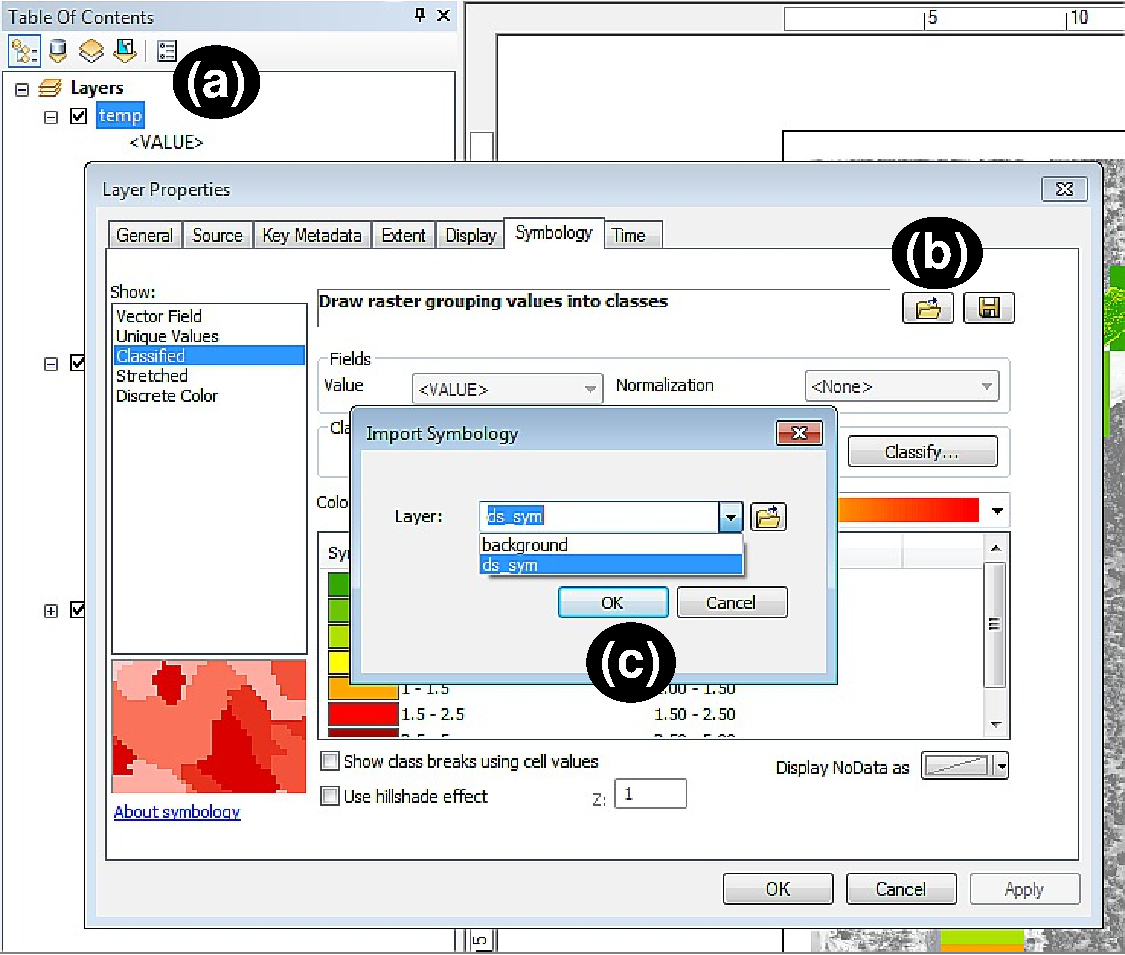
\includegraphics[width=0.75\columnwidth]{make_layouts.pdf} % Example image
	\caption{Steps~a) to~c) for adapting the symbology in \textit{ArcGIS Desktop} according to the descriptions in the text.\label{fig:make_layouts}}
\end{figure}

The module uses layouts that are placed in the directory \texttt{.../Output/Mapping/.ReferenceLayouts/}, which should not be changed unless the \texttt{pdf} style requires adaptations. The map extents, scales and focus can be changes in the \texttt{mapping.inp} file (see Sec.~\ref{sec:inpmaps}).

\subsubsection{Interpretation}
The success of features corresponds to their ecological sustainability and physical stability, which may positively correlate, i.e., high stability corresponds to high ecological sustainability. However, features such as gravel augmentation or grading have an inverse relationship between ecological sustainability and physical stability. For example, frequently mobile gravel injections create valuable habitat but are, by definition, unstable. In such cases, the lifespan maps need to be considered in the opposite way: Optimum areas for application correspond to regions with low lifespans.

\subsubsection{Quit module and logfiles}
The GUI can be closed via the \texttt{Close} dropdown menu if no background processes are going on (see terminal messages). The GUI flashes and rings a system bell when it completed a run task. If layout creation and/or mapping were successfully applied, the target folder automatically opens. After execution of either run task, the GUI disables functionalities, which would overwrite the results and it changes button functionality to open logfiles and quit the program. Logfiles are stored in the \texttt{RiverArchitect/LifespanDesign/} folder with names \texttt{lifespan{\myUnderscore}design.log} (Raster Maker) and \texttt{mapper.log} (Layout/Map Maker). Logfiles from the previous runs are overwritten.

%----------------------------------------------------------------------------------------


\section{Parameter hypothesis} \label{sec:par}
% \subsection{List of parameters}
Combinations of recurring parameters determine the lifespans of features. The code analyses the following parameters, where the application order (hierarchy) differs from the alphabetic order for reasons of map integrity (see coding conventions in Sec.~\ref{sec:order} for details).
\begin{itemize}
	\item \texttt{chsi} composite Habitat Suitability Index (dimensionless value between 0 and 1)
	\item \texttt{d2w} is the surface depth to the groundwater table (length units)
	\item \texttt{det} is the detrended DEM (length units)
	\item \texttt{Dcr} are mobile or stable grain sizes that are entrained by rare discharges that occur according to a defined return period (see angular boulders (rocks) in Sec.~\ref{sec:rocks}
	\item \texttt{fill} corresponds to annual sediment deposition rates \citep[length units; see also][]{wyrick16}
	\item \texttt{Fr} is the Froude number corresponding to \texttt{u}/(\texttt{h}~$g$), where $g$ denotes gravity acceleration (dimensionless hydraulic)
	\item \texttt{h} is the flow depth (length units)
	\item \texttt{mu} are the morphological units \citep[strings; see also][]{wyrick14b}
	\item \texttt{Se} is the energy slope (cf. angular boulders (rocks) in Sec.~\ref{sec:rocks} and side channels in Sec.~\ref{sec:sidechnl})
	\item \texttt{scour} corresponds to annual erosion rates \citep[length units, see also][]{wyrick16}
	\item \texttt{sidech} delineation of priority regions for side channels \citep{vandenderen17}
	\item \texttt{taux} (or $\tau_*$) is the dimensionless bed shear stress and its critical value $\tau_{*,cr}$ (--)
	\item \texttt{tcd} combines \texttt{scour} and \texttt{fill} analysis
	\item \texttt{u} is the flow velocity (length per time, i.e., fps or m/s)
	\item \texttt{wild} wildcard parameter that can only take on/off values (noData, 0 or 1)
\end{itemize}

The code uses the \texttt{mu} raster to identify feature-adequate morphological units that are stored in \pythoninline{feature.mu_good} and feature-inadequate units that are stored in \pythoninline{feature.mu_bad}. Thus, two approaches are possible: an inclusive approach that limits relevant areas using the \pythoninline{feature.mu_good} list and an exclusive approach that excludes non-relevant areas using the \pythoninline{feature.mu_bad} list. The following morphological units are considered \citep{wyrick14b}:\\
\begin{tabular}{p{0.9cm} l L{0.295\textwidth} l l  L{0.29\textwidth}}
	\multicolumn{6}{l}{}\\ % add vspace using an empty row
	&-- & agriplain & &-- & bank \\
	&-- & bedrock  & &-- & chute \\
	&-- & cutbank & &-- & fast glide\\
	&-- & flood runner & &-- & floodplain\\
	&-- & high floodplain & &-- & hillside \\
	&-- & island high floodplain & &-- & island-floodplain\\
	&-- & lateral bar & &-- & levee\\
	&-- & medial bar & &-- & mining pit\\
	&-- & point bar & &-- & pond\\
	&-- & pool & &-- & riffle\\
	&-- & riffle transition & &-- & run\\
	&-- & slackwater & &-- & slow glide\\
	&-- & spur dike & &-- & swale\\
	&-- & tailings & &-- & terrace\\
	&-- & tributary channel & &-- & tributary delta\\
	&-- & \multicolumn{4}{l}{in-channel bar (all within-bankfull bars)}\\
	\multicolumn{6}{l}{}\\ % add vspace using an empty row
\end{tabular}

%\subsection{Habitat suitability assessment}\label{sec:hab}
%
%The application of ``habitat matching'' limits the application of all analyzed features to regions where the composite habitat suitability index (CHSI) is smaller than~0.4. The CHSI values are stored in the input raster \texttt{max{\myUnderscore}chsi} and they represent the maximum CHSI value of the following species and life stages:
%\begin{itemize}
%	\item Chinook Salmon: Spawning (CHSI5c), Fry (CHSI) and Juvenile (CHSI);
%	\item Lamprey: Adult (CHSI12)
%	\item Oncorhynchus mykiss (rainbow trout): Fry (CHSI) and Juvenile (CHSI);
%	\item Steelhead trout (CHSI12)
%	\item Sturgeon: Spawning (CSI)
%\end{itemize}
%
%Moreover, the fish species-related values correspond to the maximum CHSI of the following list of discharges in cubic feet per second (hint: not all discharge bins are available for all species and life stages):\\
%\begin{tabular}{p{0.9cm} l r r l r r l r l r r}
%	\multicolumn{12}{l}{}\\ % add vspace using an empty row
%	&-- & 300 & &-- & 350 & &-- & 400 & &-- & 450\\
%	&-- & 530 & &-- & 600 & &-- & 622 & &-- & 700\\
%	&-- & 800 & &-- & 880 & &-- & 930 & &-- & 1,000\\
%	&-- & 2,000 & &-- & 3,000 & &-- & 4,000 & &-- & 5,000\\
%	&-- & 7,500 & &-- & 10,000 & &-- & 15,000 & &-- & 21,100\\
%	&-- & 30,000 & &-- & 42,200 & &-- & 84,400 & &-- & 110,400\\
%	\multicolumn{12}{l}{}\\ % add vspace using an empty row
%\end{tabular}


\section{Feature hypothesis} \label{sec:feat}

The \textit{River Architect} package applies the following hypothesis to habitat enhancement features referring to the base case of the lower Yuba River in its 2008 condition. For the topographic change, scour and fill rates are considered over a six-year observation period \citep[2008 to 2014, see][]{weber17}. The base case stores the below stated threshold parameters in \texttt{RiverArchitect/LifespanDesign/.templates/threshold{\myUnderscore}values.xlsx}.

\subsection{Backwater}\label{sec:backwtr}
The creation of artificial backwaters and swales, or more generally calm water zones, makes sense where the stream power is low and the observed topographic changes are small. The following parameters identify relevant areas for backwater creation:
\begin{itemize}
	\item \texttt{u} with a threshold of 0.1~fps (0.03~m/s).
	\item \texttt{mobile{\myUnderscore}grains} with frequency threshold of 4.7~years and $\tau_{*,cr}$ threshold of 0.047.
	\item \texttt{tcd} with scour and fill thresholds of $\geq$~0.1~ft$\cdot$6~years.
	\item \texttt{mu} using the inclusive method with \pythoninline{mu_good = ["agriplain", "backswamp", "mining pit", "pond", "pool", "slackwater", "swale"]}.
\end{itemize}

\subsection{Bioengineering}\label{sec:bioeng}

Areas with a 1.0-year lifespan require bioengineering features that are independent of the depth to the groundwater table because plantings likely will not have sufficient water to survive. Such features typically imply the placement of angular boulders.

In the context of river engineering, soil-bioengineering applies living materials (plants) to stabilize terrain and enhance habitat. Alas, dry conditions in arid and semi-arid (Mediterranean) climate zones limits the possibilities of application. The LifespanDesign module maps potential bioengineering areas, as a function of
\begin{itemize}
	\item \texttt{d2w} the maximum depth to groundwater distance indicates where vegetation plantings-based bioengineering applies.
	\item \texttt{dem} is used to compute the percentwise terrain slope \texttt{S0}, where modified terrain with slopes of more than a certain percentage is considered to require reinforcement (set \texttt{S0} threshold in \texttt{RiverArchitect/Lifespan Design/.templates/threshold{\myUnderscore}values.xlsx}, see Sec.~\ref{sec:modthresh})
\end{itemize}

The lifespan maps of bioengineering features can take three values:
\begin{itemize}
	\item[] \texttt{\textbf{20.0}} years (or maximum value as defined in the input definitions file, cf. Sec.~\ref{sec:inpras}), if the terrain slope is greater than defined in the thresholds workbook and the depth to groundwater is lower than defined in the thresholds workbook (cf. Sec.~\ref{sec:modthresh});
	\item[] \texttt{\textbf{1.0}} year, if the terrain slope is greater than defined in the thresholds workbook and the depth to groundwater is greater than defined in the thresholds workbook;
	\item[] \texttt{\textbf{NoData}}, if the terrain slope is lower than defined in the thresholds workbook.
\end{itemize}


\subsection{Berm Setback / Widen}\label{sec:berms}
Berms are artificial lateral confinements that are represented by human-made bars and dikes. Also, levees represent a lateral confinement but their flood protection-function should not be deleted, and therefore, levees are not considered for setback action. The code replaces the keyword ``Bermsetback'' with ``Widen'' because the removal of lateral confinements represents a river widening.
\begin{itemize}
%	\item \texttt{mobile{\myUnderscore}grains} with $\tau_{*,cr}$ threshold of 0.047.
%	\item \texttt{tcd} with scour threshold 0.1~ft~$\cdot$~6~years and fill threshold 0.1~ft~$\cdot$~6~years.
	\item \texttt{mu} using the inclusive method with \pythoninline{mu_good = ["bank", "floodplain", "high floodplain", "island-"}\\
	\pythoninline{"floodplain", "island high floodplain", "lateral bar", "levee", "spur dike", "terrace"]}.
	\item \texttt{det} detrended DEM with a lower limit of 17~ft (5.18~m) and an upper limit of 25~ft (7.62~m).%according to the following observations:\\
%			\pythoninline{lateral bar} corresponds to \texttt{det}~$\in$~[10~ft, 30.0~ft]\\
%			\pythoninline{spur dike} corresponds to \texttt{det}~$\in$~[10~ft, 30.0~ft]
\end{itemize}
%The \pythoninline{mobile{\myUnderscore}grains} and the \pythoninline{tcd} analyses indicate bars or dikes that cannot be removed by floods. Therefore, the setback of berms makes sense where even high floods cannot erode the lateral confinements.\\

The complete detrended DEM range of the morphological unit \pythoninline{lateral bar} covers values between -1.24~ft (0.38~m) to 29.5~ft (9.0~m) and the morphological unit \pythoninline{spur dike} covers \texttt{det}-values between 1.9~ft (0.58~m) to 25.9~ft (7.89~m). The other morphological units are in similar ranges. However, the detrended DEM limits the application of berm setback and widening to economically reasonable extents. The \texttt{det} limits in the code refer to empiric values corresponding to berm setback features according to \citep{ycwa16}.


\subsection{Engineered Log Jams / Instream wood}\label{sec:ejl}
Lifespan maps and design maps are created for engineered log jams (ELJs), where the following parameters apply:

\begin{itemize}
	\item[] Lifespan maps
	\item \texttt{h} with mobility threshold of 1.7 multiplied with the log diameter of 2~ft \citep[0.6~m][]{lange06, ycwa16}.
	\item \texttt{Fr} with a threshold of 1 (critical flow conditions).
	\item \texttt{mu} excluding tributary sections (see below descriptions).
	\item[] Design maps
	\item \texttt{h} is used to computed the minimum required log diameter to avoid motion for a 20-years flood.
\end{itemize}

Regarding morphological units, riffle-pool and plane bed morphologies are favorable for ELJ placement, where side channel and tributary systems are not convenient for wood placement. ELJs inclusive list is defined as \pythoninline{mu_good = ["riffle", "riffle transition", "pool", "floodplain", "island floodplain", "lateral bar", "medial bar",}\\
\pythoninline{" run"]} and the exclusive list is defined as \pythoninline{mu_bad = ["tributary channel", "tributary delta"]}. For ELJs, the exclusive approach based on \pythoninline{mu_bad} applies (see details in the parameter descriptions in Sec.~\ref{sec:par}).\\

The design maps for the minimum required log diameter~$D_w$ result from \citep{ruiz16b}'s interpolation curve as a function of the flow depth. The module applies on the single-thread formula because it returns larger values for the log diameter than the multi-thread formula when the probability of motion is set to zero: \texttt{Dw}~=~0.32~/~0.18~$*$~\texttt{h}. The output map limits to regions where \texttt{Dw} is smaller than 300~in (7.6~m).

\subsection{Fine sediment}\label{sec:finesed}
Artificially introduced fine sediment facilitates root growth of new plantings but the flow may easily entrain artificially placed fine sediment. Moreover, spontaneous percolation of fine sediment into the voids of the coarser existing sediment may occur. Therefore, plantings-specific parameters apply to the introduction of fine sediment, as well as filter criteria. The analysis considers fine sediment with a maximum grain diameter of 0.08~in (2~mm sand). The \pythoninline{feature analysis} module uses the following raster criteria:

\begin{itemize}
	\item[] Lifespan maps
	\item \texttt{taux} with a threshold of $\tau_{*,cr}$~=~0.030.
	\item \texttt{Dcf} is the maximum admissible size of fine sediment including the ($D_{max, fine}~<$~0.08~in [2~mm]).
	\item \texttt{tcd} with the scour threshold of White Alder (largest for plantings) of 1~ft (0.308~m) multiplied with 6~years and the fill threshold of Cottonwood (highest for plantings) of 0.8$\cdot$0.2$\cdot$7~ft [2.13~m]$\cdot$6~years
	\item \texttt{d2w} with a lower limit of 1~ft and an upper limit of 10~ft corresponding to plantings limits.
	\item[] Design maps
	\item \texttt{filter} criteria resulting in a design map according to \citep{usace00}:\\
			$D_{15, fine}~>~D_{15, coarse}$~/~20;\\
			$D_{85, fine}~>~D_{15, coarse}$~/~5;\\
			$D_{max, fine}$ must be finer than sand, i.e., $<$~0.08~in (2~mm), to satisfy its ``fine'' character.
\end{itemize}

The topographic change and depth to water table thresholds correspond to the largest values that any plantings type (cf. Sec.~\ref{sec:plants}) supports because only these areas are of interest for the incorporation of fine sediment in soils.

\subsection{Grading}\label{sec:grading}
Grading aims at the reconnection of high floodplains and isolated islands by means of floodplain terracing and bar lowering. Its application is from an interest in areas where potential plantings cannot reach the groundwater table or where even high discharges cannot rework the channel. Low dimensionless shear stress, infrequent grain mobilization or low scour rates indicate relevant sites. The following parameter rasters and hypothesis apply to lifespan maps for grading measures (no design maps).
\begin{itemize}
	\item \texttt{mobile{\myUnderscore}grains} with frequency threshold of 12.7~years and $\tau_{*,cr}$ threshold of 0.047.
	\item \texttt{taux} with mobility threshold of $\tau_{*,cr}$ equal to 0.047.
	\item \texttt{scour} with a threshold value of 0.1~ft multiplied with 6 years and the inverse argument, i.e., areas of interest correspond to regions where the scour threshold is not exceeded.
	\item \texttt{d2w} with a lower limit of 7~ft (2.13~m) and an upper limit of 10~ft (3.05~m).
\end{itemize}

Further aspects may be considered in addition to the implemented parameters:
\begin{itemize}
	\item Depth to groundwater\\
	The YRERFS report \citep{ycwa16} proposes grading where the depth to groundwater is between 7 (2.13~m) and 10~ft (3.05~m). A visual control of the maps indicates that the upper limit should be increased to 12~ft which corresponds to the tip of several islands.
	\item Morphological Units\\
	Currently not applied because every analysis would require the expensive manual assessment of morphological units. This is not necessary for assessing potential grading zones that are primarily determined by the depth to groundwater.
\end{itemize}

\subsection{Plantings}\label{sec:plants}
The survival analysis of plantings assumes a general cutting length of min. 7 ft (2.13~m), where approximately 80~$\%$ of the cuttings are planted in the ground and 20~$\%$ protrude above the ground. The lifespan maps for plantings vary among four indigenous species, which have previously been determined to be relevant for habitat enhancement at lower Yuba River. No design maps are created because the lifespan maps already contain all relevant information.
\begin{itemize}
	\item Box Elder\\
	Parameters \citep[extracted from][]{friedman99, kui16a}: \texttt{h} (exclude all submerged regions for more than 1'000~cfs), \texttt{taux} (threshold of 0.047) and \texttt{d2w} (lower threshold is 3~ft and upper threshold is 6~ft);\\
	The maximum submergence duration supported by Box Elder cuttings is 85 days per year. The discharge duration curve from Marysville gaging station (1967--2015) indicate a cumulative annual submergence of 85 days per year for a discharge of 569~cfs, where the Hallwood-study indicates successive 21-submergence when the discharge exceeds 2'000~cfs. The code uses the 1'000-cfs-discharge situation as tradeoff for the 85-days submergence criterion.
	\item Cottonwood\\
	Parameters \citep[extracted from][]{stromberg93, polzin06, wilcox13, bywater15, kui16a}: \texttt{hyd} ($h~\geq$~1.5$\cdot$0.2$\cdot$7~ft [2.13~m] and $u~\geq$~3.0~fps), \texttt{tcd} (scour$\geq$ 0.1$\cdot$0.8$\cdot$7~ft [2.13~m] $\cdot$6 years and fill $\geq$~0.8$\cdot$0.2$\cdot$7~ft$\cdot$6 years) and \texttt{d2w} (lower threshold is 5~ft and upper threshold is 10~ft);\\
	Uses thresholds for combined hydraulics analysis (velocity and depth), scour and fill (tcd) and depth to water table. Given the minimum cutting length of 7~ft (2.13~m), cottonwood plantings have a \pythoninline{threshold_scour} of 0.1$\cdot$0.8$\cdot$7~ft$\cdot$6 years (2008 to 2014) and a \pythoninline{threshold_fill} of 0.8$\cdot$0.2$\cdot$7~ft$\cdot$6~years.
	\item White Alder\\
	Parameters: \texttt{taux} (threshold of 0.047), \texttt{scour} \citep[$\geq$~1~ft$\cdot$6~years, cf.][]{jablkowski17} and \texttt{d2w} (lower threshold is 1~ft and upper threshold is 5~ft);\\
	In addition to the scour maps, potential scour resulting from a grain mobility frequency analysis provide information on the lifespans of White Alder plantings. \pythoninline{threshold_scour} is 1~ft$\cdot$6~years.
	\item Willow\\
	Parameters \citep[extracted from][]{stromberg93, pasquale11, pasquale12, pasquale14}: \texttt{h} ($h~\geq $~0.7~ft~+~0.2$\cdot$7~ft), \texttt{taux} (threshold of 0.1), \texttt{scour} ($\geq$~0.1$\cdot$0.8$\cdot$7~ft$\cdot$6~years) and \texttt{d2w} (lower threshold is 3~ft and upper threshold is 5~ft);\\
	Willow cuttings have a maximum submergence survival that defines the \pythoninline{threshold_h} as 0.7~ft~+~0.2$\cdot$7~ft and maximum scour survival of 0.1$\cdot$0.8$\cdot$7~ft$\cdot$6~years.
\end{itemize}

\subsection{Angular boulders (rocks)}\label{sec:rocks}
The punctual placing of boulders and comprehensive rock cover is referred to as ``angular boulders (rocks)'' for stabilizing banks or erosion-prone surfaces \citep[e.g.,][]{maynord08}. The mobility of the present terrain indicates the necessity of boulder placement on the basis of lifespan maps. Moreover, the required minimum diameter for boulders results from the spatial evaluation of $D_{cr}$ on angular boulders (rocks) design maps. The following parameters apply to the generation of angular boulders (rocks) maps:
\begin{itemize}
	\item[] Lifespan maps
	\item \texttt{taux} with mobility threshold of $\tau_{*,cr}$ equal to 0.047.
	\item \texttt{scour} with a threshold value of 1~ft multiplied with 6 years.
	\item[] Design maps
	\item \texttt{stable{\myUnderscore}grains} for design maps (see below formulae), with a frequency threshold of 20.0~years and $\tau_{*,cr}$ threshold of 0.047.
\end{itemize}

The minimum required grain sizes are determined in a two-way analysis, i.e., two minimum angular boulders (rocks) size maps are produced based on the highest discharge where hydraulic data is available (20.0 years):
\begin{enumerate}
	\item \texttt{ds{\myUnderscore}rocks{\myUnderscore}Dcr} is a derivative of the Gauckler-Manning-Strickler formula using Manning's $n$:\\
	$D_{cr}$ = \textit{SF}~$\cdot u^2 \cdot n^2$~/~$\left[\left(s - 1\right) \cdot h^{1/3} \cdot \tau_{*,cr} \right]$
	\item \texttt{ds{\myUnderscore}rocks{\myUnderscore}Dcr} is a derivative of the Ch\'ezy formula using the energy slope:\\
	$D_{cr}$ = \textit{SF}~$\cdot h \cdot S_e$~/~$\left[\left(s - 1\right) \cdot \tau_{*,cr} \right]$
\end{enumerate}
where:
\begin{itemize}
	\item[$D_{cr}$] is the minimum required angular boulders (rocks) size (in INCHES);
	\item[$h$] is the flow depth (pixel-wise, in ft);
	\item[$n$] is Manning's n (in s/ft$^{1/3}$ -- an internal conversion factor of k = 1.49 applies);
	\item[$s$] is the dimensionless relative grain density (ratio of sediment and water density, equal to 2.68);
	\item[$S_e$] is the energy slope (derived from \pythoninline{arcpy}'s ``Slope'' function, dimensionless);
	\item[\textit{SF}] is a safety factor equal to 1.3 (dimensionless);
	\item[$u$] is the flow velocity (pixel-wise, in fps);
	\item[$\tau_{*,cr}$] is the threshold value of dimensionless bed shear stress for incipient grain motion, equal to 0.047.
\end{itemize}
The energy slope maps result from computing the theoretic energy height maps as \pythoninline{ras_energy} = \pythoninline{dem} + \pythoninline{h.raster_110k} + \pythoninline{u.raster_110k}$^2$/(2~$g$), where $g$ denotes gravitational acceleration.

\subsection{Sediment replenishment / gravel augmentation}\label{sec:gravel}
Large dams tend to retain the nearby-totality of the catchment sediment supply. The missing sediment causes channel incision and the morphological depletion of lower Yuba River in the long term. Regular artificial gravel injections can antagonize this artificial sediment scarcity \citep[e.g.,][]{pasternack10a}. Other authors (\citep{gaeuman08} and \citep{ock13}) distinguish replenishment techniques inside and outside of the main channel. According to this, two types of gravel augmentation are considered:
\begin{enumerate}
	\item Gravel stockpiles on the floodplain and river banks; and
	\item Gravel injections or stockpiles directly in the main channel.
\end{enumerate}
Gravel deposits on floodplains should be erodible by frequent floods, i.e., stockpiles make sense where only larger floods entrain grains. In contrast, gravel injections in the main channel aim at the immediate creation of spawning habitat that should not wash out with the next minor flood event. However, gravel injections with low longevity in the main channel can also serve for an urgent equilibrium of river sediment budget. Therefore, the lifespan maps for gravel replenishment require two different interpretations inside and outside of the main channel: High lifespans are desirable in the main channel for immediate habitat creation and low lifespans are desirable for equilibrating the sediment budget.
\begin{itemize}
	\item In-channel gravel injections
	\begin{itemize}
	\item[] Lifespan maps
	\item \texttt{mobile{\myUnderscore}grains} analysis with a minimum frequency of 1.0~years and $\tau_{*,cr}$ threshold of 0.047.
	\item \texttt{mu} uses the inclusive method with \pythoninline{mu_good = ["chute", "fast glide", "flood runner", "bedrock", "lateral bar", "medial bar", "pool", "riffle", "riffle transition", "run", "slackwater", }\\
	\pythoninline{"slow glide", "swale", "tailings"]}
	\item[] Design maps
	\item \texttt{stable{\myUnderscore}grains} for design maps (see angular boulders (rocks) formulae), with \pythoninline{threshold_freq} of 1.0~years and $\tau_{*,cr}$--threshold of 0.047.
	\end{itemize}
	\item Floodplain / overbank gravel stockpiles
	\begin{itemize}
	\item[] Lifespan maps
	\item \texttt{mobile{\myUnderscore}grains} analysis with a minimum frequency of 1.0~years and $\tau_{*,cr}$ threshold of 0.047.
	\item \texttt{scour} with a threshold value of 1~ft per year.
	\item \texttt{mu} uses the inclusive method with \pythoninline{mu_good = ["agriplain", "backswamp", "bank", "cutbank", "flood runner", "floodplain", "high floodplain", "hillside", "island high floodplain", "island-"}\\
	\pythoninline{"floodplain", "lateral bar", "levee", "medial bar", "mining pit", "point bar", "pond", "spur"}\\
	\pythoninline{"dike", "tailings", "terrace"]}
	\item[] Design maps
	\item \texttt{stable{\myUnderscore}grains} for design maps (see angular boulders (rocks) formulae), with \pythoninline{threshold_freq} of 1.0~years and $\tau_{*,cr}$--threshold of 0.047.
	\end{itemize}
\end{itemize}

\subsection{Side cavities}\label{sec:sidecav}
From a parametric point of view, side cavities make sense at lateral channel confinements that represent either preservable habitat or require protection to prevent bank collapses. In the latter case, groin cavities are an adequate protection measure that can additionally improve habitat conditions. The code analyses relevant sites based on the morphological units and important scour rates at banks. It excludes fill zones where artificial side cavities are prone to sedimentation making the measure ecologically inefficient.

\begin{itemize}
	\item \texttt{tcd} with a fill threshold value of 1~ft multiplied with 6 years and a scour threshold of 100~ft leads to the exclusion of fill-prone sites.
	\item \texttt{mu} using the inclusive method with \pythoninline{mu_good = ["bank", "cutbank", "lateral bar", "spur dike", "tailings"]}.
\end{itemize}


\clearpage
\subsection{Side channels / anabranches}\label{sec:sidechnl}
Any discrete parameters exist for assessing design or lifespan maps for side channels, anabranches, anastomosed or multithread channels. The identification of splays and bank rigidity requires manual and visual proof.\\

An initial decision support on the basis of design maps was contemplated by comparing the minimum energy slope~$S_{e,min}$ with the terrain slope$S_0$. In the 1D-theory, the minimum energy slope results from the $H$-$h$ diagram \citep{glenn15}, based on the assumption that the minimum energy per unit force and pixel~$H_{min}$ corresponds to the Froude number~$Fr$~=~1 with the critical flow velocity~$u_c$ and flow depth~$h_c$. The pixel unitary discharge results from $q$~=~$u~\cdot h$, where $u$ and $h$ are pixel values from the \texttt{u} and \texttt{h} rasters. Thus, the following system of equations can be used:
\begin{subequations}
\begin{flalign}
&Fr &=&\hspace{0.25cm} 1 &\leftrightarrow \hspace{0.25cm} &1 = \frac{u_c}{\sqrt{g~h_c}} &\hspace{0.25cm}\leftrightarrow& \hspace{0.25cm}u_c = \sqrt{g~h_c}& \hspace{5.0cm}\label{eq:Fr} \\
&h_c &=&\hspace{0.25cm} \left(\frac{q^2}{g}\right)^{1/3} &&&&\label{eq:hc}\\
&q &=&\hspace{0.25cm} u \cdot h &&&&\label{eq:q}\\
\Rightarrow \hspace{0.25cm}&H_{min} &=&\hspace{0.25cm} h_c + \frac{u_c^2}{2~g} &\hspace{0.25cm}=\hspace{0.25cm}& 1.5\cdot \left(\frac{q^2}{g}\right)^{1/3}&&&\label{eq:Hmin}
\end{flalign}
\end{subequations}

Thus, the available discharges and related flow velocity~\texttt{u} / depth~\texttt{h} rasters could be used for the following calculation (python script sample):\\
\begin{python}
S0 = Slope(dem.raster, "PERCENT_RISE", 1.0))/100
for h.ras in h.rasters and u.ras in u.rasters:
          ## compute energetic level
          energy_level[discharge] = dem.raster + 1.5 * Power(Square(h.ras[discharge] * u.ras[discharge]) / g, 1/3)})
          ## compute energy slope Se,min
          Se[discharge] = Slope(energy_level[discharge], "PERCENT_RISE", 1.0))/100
          ## result = compare Se and S0 (Se / S0)
          Se_S0[discharge] = Se[discharge] / S0)})
\end{python}

This sample function uses \texttt{arcpy.sa}'s \texttt{Slope} function with the arguments \texttt{PERCENT{\myUnderscore}RISE} for obtaining percent values instead of degrees and \texttt{zFactor}~=~1.0 because the x-y-grid units are the same as in z-direction. \texttt{g}~denotes gravity acceleration (SI metric: 9.81~m/s$^s$ or U.S. customary: 32.2~ft/s$^2$).\\
However, the underlying 2D numerical model uses the critical flow depth as an iteration criterion for stability, which causes that $S_{e,min}$ approximately equals $S_{0}$. Thus, the $S_{e,min}$ / $S_{0}$ ratio is approximately unity and not meaningful. Otherwise, the  $S_{e,min}$ / $S_{0}$ indicated pixels with excess energy ($S_{e,min}$~/~$S_0~>$~1) that allegedly caused erosion. In contrast, pixels with energy shortage ($S_{e,min}$~/~$S_0~<$~1) allegedly resulted in sediment deposition. Minor topographic change would be expected where the $S_{e,min}$~/~$S_0$--ratio is close to unity.\\% The resulting design maps would be named \texttt{ds{\myUnderscore}sidechn{\myUnderscore}XXX} where \texttt{XXX} represents the three-digits discharge in thousand~cfs. 
Unless this problem is not solved, the package indicates the adequacy of side channel construction on lifespan maps using the following criteria:
\begin{itemize}
	\item \texttt{fill} the fill rate does not exceed the threshold value defined in the thresholds spreadsheet (Sec.~\ref{sec:modthresh})
	\item \texttt{taux} the critical dimensionless bed shear stress should be smaller than the threshold value defined in the thresholds spreadsheet (Sec.~\ref{sec:modthresh})
	\item \texttt{sidech} needs to be a manually created \textit{Arc GRID} raster in \texttt{01{\myUnderscore}Conditions/\textit{condition}/}. The delineation is typically made in a shape file, which is then converted into an \textit{Arc GRID} raster file. The delineation criteria are \citep{vandenderen17}:
	\begin{itemize}
		\item Side channel intakes are situated at the outer bank, downstream of outer bends or at the inner bank, inside mild inner bends;
		\item A side channel should be longer than the main channel to avoid cutting off the main channel;
		\item Structures should be placed in the side channel to control the flow repartitioning and to avoid flow separation in the main channel.
	\end{itemize}
\end{itemize}
Moreover


\section{Input definition files}\label{sec:inp}
\subsection{Raster data}\label{sec:inpfile}

The file \texttt{input{\myUnderscore}definitions.inp} is stored on the directory \texttt{/.templates/} and can be accessed using the link \texttt{InputDefinitions.lnk} directly in the code directory. \texttt{input{\myUnderscore}definitions.inp} contains information about lifespan duration and raster names, which link to rasters containing spatial information as described in Sec.~\ref{sec:par}. The order of definitions and lines must not be changed to ensure the proper functioning of the module. Enter or change information in the corresponding lines, only between the ``='' and the ``$\#$'' signs (the input routines uses these signs as start and end identifiers for relevant information). The following definitions apply line by line:\\

\begin{tabular}{l p{0.2\textwidth} L{0.65\textwidth}}
\multicolumn{3}{l}{}\\
Lines 1--3 & None &Do not change\\ \rowcolor{med_gray}
Line  4 & Return periods & Comma-separated list of flood discharge return periods corresponding to the hydraulic rasters; i.e., the first entry after ``='' corresponds to the return period of the first velocity and flow depth raster (Lines 11 and 12, respectively)\\
Lines 5--7 & None &Do not change\\ \rowcolor{med_gray}
Line  8 & CHSI & One raster name of spatial composite Habitat Suitability Indexes \\
Line  9 & DoD  & Comma-separated list of two (first = scour, second = fill) DEM of Differences rasters; if one raster is missing, replace it by double quotation marks, for example scour is missing: \pythoninline{... = "", dodFill # ...}\\ \rowcolor{med_gray}
Line 10 & det  & One raster name defining the detrended DEM raster\\
Line 11 & u		 & Comma-separated list defining flow velocity rasters corresponding to discharge return periods (Line~4); replace missing rasters by double quotation marks, for example, when \texttt{u} rasters of a return period list of five entries are not available for entries 2 and 4, type \pythoninline{... = u001k, "", u003k, "", u005k # ...}. However, ensure that at least two \texttt{u} rasters are defined. The \pythoninline{00xk} identifier relates to the underlying discharge in thousand cfs or m$^3$/s. Smaller discharges are written without "\texttt{k}". For example, a velocity raster related to a discharge of 110423~cfs is named \pythoninline{u110k}, and a velocity raster related to a discharge of 544.4~cfs  is named \pythoninline{u544}.\\ \rowcolor{med_gray}
Line 12 & h		 & Comma-separated list defining flow depth rasters corresponding to discharge return periods (Line~4); replace missing rasters by double quotation marks, for example, when \texttt{h} rasters of a return period list of six entries are not available for entries 2, 3 and 5, type \pythoninline{... = h001k, "", "", h004k, "", h006k # ...}. Ensure that at least two \texttt{h} rasters are defined. The \pythoninline{00xk} identifier relates to the underlying discharge in thousand cfs or m$^3$/s. Smaller discharges are written without "\texttt{k}". For example, a flow depth raster related to a discharge of 110423~cfs is named \pythoninline{h110k}, and a flow depth raster related to a discharge of 544.4~cfs  is named \pythoninline{h544}.\\
Line 13 & Grains& One raster name defining the raster containing mean grain diameters (pay attention on raster units: use feet for U.S. customary and m for S.I.)\\ \rowcolor{med_gray}
Line 14 & mu  & One raster name delineating morphological units according to the definitions in Sec.~\ref{sec:par}\\
Line 15 & d2w & One raster name defining the depth to groundwater table\\ \rowcolor{med_gray}
Line 16 & DEM & One raster name defining the digital elevation model\\
Line 17 & sidech & One raster name delineating appropriate sites for side channels\\ \rowcolor{med_gray}
Line 18 & wild & One raster name for the spatial confinement of the feature analysis of 0/nodata (= off) and 1 (= on) values for any purpose (wildcard raster)\\
\multicolumn{3}{l}{}\\
\end{tabular}

The module produces results based on the available information only, where any raster name can be substituted with double quotation marks \pythoninline{""}. However, this lack of information reduces the accuracy of final lifespan and design maps. No maps are produced for a feature where the information is insufficient for the analysis. The required information for every feature corresponds to the definitions in Sec.~\ref{sec:inpfile}.

\subsection{Mapping}\label{sec:inpmaps}
The file \texttt{mapping.inp} defines map center points, extents ($dx$ and $dy$ in ft) and scales (scale has no effect currently). \texttt{mapping.inp} is stored on the directory \texttt{/.templates/} and directly accessible from the code directory via the link \texttt{MapLayouts.lnk}.\\

The extent of the map determines the map scale, where the corresponding $dx$ and $dy$ values define the map width and height in ft, respectively. The layout templates (\texttt{.mxd} in the directory \texttt{.../Output/Mapping/.Reference Layouts/} define the paper size, which is by default ``ANSI E landscape'' (width = 44~inches, height = 34~inches).\\
The map focus is defined page-wise in \texttt{mapping.inp} from Line~8 onward. Existing pages can be removed by simply deleting the line. Additional pages can be added by inserting or appending a new line below Line~8, which needs to begin with the keyword ``\texttt{Page}'' and $x$ and $y$ need to be stated in brackets, separated by a comma without any white space (\pythoninline{[xxxxxx.xx,yyyyyy.yy]}).\\

Good practice for changing the map layouts starts with opening the \texttt{find{\myUnderscore}center{\myUnderscore}points.mxd} layout from \texttt{.../Output/Mapping/.ReferenceLayouts/}. Zoom to new focus point using, for example, \textit{ArcGIS} \texttt{Go To XY} function from the \texttt{Tools} toolbar or freehand to any convenient extent. Use \textit{ArcGIS} \texttt{Info} cursor and click in the center of the reticule to obtain the current center point. Write new center point coordinates for the desired page number in \texttt{mapping.inp}.\\
For retrieving the extent, in \textit{ArcGIS} Desktop, go to the \texttt{View} menu, click on \texttt{Data Frame Properties...} and go to the \texttt{Data Frame} tab. In the \texttt{Extent} box, click on the scroll-down menu and choose \texttt{Fixed Extent}. Subtracting the \texttt{Right} value from the \texttt{Left} value defines $dx$ (Line~3 in \texttt{mapping.inp}) and subtracting the \texttt{Top} value from the \texttt{Bottom} value defines $dy$ (Line~4 in \texttt{mapping.inp}).\\
The \pythoninline{feature_analysis.map_maker()} function uses these definitions for zooming to each point defined below Line~8 in \texttt{mapping.inp}, cropping the map to the defined extents and exporting each page to a \texttt{PDF} map bundle containing as many pages as there are defined in \texttt{mapping.inp}.\\
The program uses the reference coordinate system and projection defined in the layout templates (\texttt{.mxd}); i.e., coordinate definitions in \texttt{mapping.inp} and \texttt{.mxd} files need to refer to the same coordinate system and projection.



\section{Code extension and modification} \label{sec:code}
The code can be extended with new parameters, e.g., direct shear stress output from the numerical model, new analyses, e.g., a new shear stress law, and features, e.g., another plant species block ramps.

\subsection{Conventions}
The rasters creation results from \pythoninline{analysis_} and \pythoninline{design_} functions that are stored in \texttt{cLifespanDesignAnalysis}. \pythoninline{analysis_} functions create rasters with lifespan data (0 to 20 years) and \pythoninline{design_} functions create rasters with design parameters such as the required stables grain size of angular boulders (rocks).\\
Class names start with an upper case letter and do not contain any special characters, also excluding dash or underscore signs. Instantiations of classes are all lower case letters. Features, Parameters and Analysis classes are stored in separate files called \texttt{cFeatureLifespan.py}, \texttt{cParameters.py} and \texttt{cLifespanDesignAnalysis.py}, respectively. In addition, Feature classes may inherit subfeature classes from files names \texttt{cSubfeature.py}, for example \texttt{cPlants.py}.\\
Function names consist of lower case letters only and the underscore sign ``{\myUnderscore}'' separates words.\\
All class names, variable names and function names are in alphabetic order (a = up, z = down), except the \pythoninline{parameter_list}s, which determine the run hierarchy (see Sec.~\ref{sec:order}).

\subsection{Order of analysis and temp (.cache) raster names}\label{sec:order}
The best position of restoration features and their lifespans depend on multiple parameters in most cases. The output rasters (lifespan maps) are computed in by batch-processing every parameter, i.e., one parameter map is processed after another. This batch processing strictly follows the below-listed hierarchy:
\begin{enumerate}
	\item Flow depth rasters (dimensional) starting with the lowest discharge to the highest discharge\\
	Internal raster name: \texttt{ras{\myUnderscore}hXXXk}
	\item Flow velocity rasters (dimensional) starting with the lowest discharge to the highest discharge\\
	Internal raster name: \texttt{ras{\myUnderscore}uXXXk}
	\item Hydraulic rasters (dimensionless)\\
	Internal raster name: \texttt{ras{\myUnderscore}taux} (dimensionless bed shear stress) or \texttt{ras{\myUnderscore}Fr} (Froude number); if needed: the hierarchy among the dimensionless hydraulic numbers is not important
	\item Mobile bed, fine sediment and stable grain size raster analysis\\
	Internal raster name: \texttt{ras{\myUnderscore}Dcr} (mobile or stable grain size) 
	\item Topographic change rasters\\
	Internal raster names: \texttt{ras{\myUnderscore}fill} (fill raster only), \texttt{ras{\myUnderscore}scour} (scour only) or \texttt{ras{\myUnderscore}tcd} (combined fill and scour)
	\item Detrended DEM raster analysis\\
	Internal raster name: \texttt{ras{\myUnderscore}det} (relevant, e.g., for berm setback)
	\item Morphological Unit rasters\\
	Internal raster name: \texttt{ras{\myUnderscore}mu}
	\item Side channel delineation\\
	Internal raster name: \texttt{ras{\myUnderscore}sch}
	\item Depth to water table\\
	Internal raster name: \texttt{ras{\myUnderscore}d2w} (relevant, e.g., for plantings and terrain grading)
\end{enumerate}

The dimensional hydraulic maps need to be invoked before any other analysis is performed because the $u$ and $h$ maps are the only ones that entirely cover the area of interest, without ``\texttt{noData}'' pixels.\\
Every \pythoninline{feature} has a \pythoninline{feature.parameter_list} attribute containing a list of parameters that determine the feature lifespan and applicability space. The parameters are ordered in the \pythoninline{feature.parameter_list} according to the hierarchy. Once the last element of \pythoninline{feature.parameter_list} is processed and stored in the cache folder, the code exits the loop and copies the last \texttt{ras{\myUnderscore}\textit{parameter}} to the \texttt{Output/Rasters/\textit{condition}/} folder. This copy is renamed \texttt{lf{\myUnderscore}\textit{shortname}}, where the usage of shortnames (see list in Sec.~\ref{sec:featoverview}) is necessary because \texttt{arcpy} cannot save or copy raster with names exceeding 13 characters.
\clearpage
\subsection{Add parameters} \label{sec:add-par}
The currently implemented parameters are listed in Sec.~\ref{sec:par}. New parameters require new input rasters in addition to the list in Sec.~\ref{sec:input}. The rasters need to be saved in the folder \texttt{01{\myUnderscore}Conditions/\textit{condition}/} using the \textit{Esri Grid} format. Other raster formats such as \texttt{.tif} may cause inconsistencies that result in error messages when the code attempts to save the final rasters. The template for creating a new parameter class is shown in the box. Use the following workflow to implement a new parameter in the code:
\begin{enumerate}
	\item Create \textit{Esri Grid} parameter rasters in the folder \texttt{01{\myUnderscore}Conditions/\textit{condition}/}.
	\item Add a new parameter class in the file \texttt{cParameters.py} (cf. box explanations).
	\item Add a new function called \texttt{analyse{\myUnderscore}\textit{parameter}} to the \texttt{ArcPyAnalysis} class in the file \\ \texttt{cLifespanDesignAnalysis.py} (see Sec.~\ref{sec:add-ana}) or change existing analysis for using the new parameter.
\end{enumerate}

\problemAnswer{
\textbf{Add new parameter class to \texttt{cParameters.py}}
\begin{itemize}
	\item[--] Replace \texttt{EXPRESSIONS} as indicated
	\item[--] Write function in alphabetic order in \texttt{cParameters.py}; e.g., the class \texttt{Mypar} should be placed below the existing class \texttt{GrainSizes} and \texttt{WaterTable}
	\item[--] Coding convention: the class name begins with a Capital letter, where an instance of the class would begin with a small letter
\end{itemize}}
%\resizebox*{1.0\textwidth}{!}{
%\begin{minipage}
\begin{python}
class PARAMETERNAME():
  def __init__(self, condition):
    self.condition=condition  # [str] planning situation, .e.g., "2008"
    self.raster_path='YOUR PATH/01_Conditions/'
    self.raster_names=['RASTER1', 'RASTER2', ..., 'RASTERi', ..., 'RASTERn']
    self.RAS1=arcpy.Raster(self.raster_path+self.condition+'/'+self.raster_names[0])
    self.RAS2=arcpy.Raster(self.raster_path+self.condition+'/'+self.raster_names[1])
    ...
    self.RASi=arcpy.Raster(self.raster_path+self.condition+'/'+self.raster_names[i-1])
    ...
    self.RASn=arcpy.Raster(self.raster_path+self.condition+'/'+self.raster_names[n-1])
\end{python}
%\end{minipage}%}

\clearpage
\subsection{Add analysis} \label{sec:add-ana}
The analysis routines are differentiated between \pythoninline{analyse} and \pythoninline{design}-functions, which are contained in the file \\\texttt{cLifespanDesignAnalysis.py}.\\
\pythoninline{analyse}-functions return rasters containing estimated survival times (in years) or on/off values (1/0). An \pythoninline{analyse}-function will always try to find existing rasters produced from previous analysis functions according to the analysis hierarchy (Sec.~\ref{sec:order}), unless a dimensional hydraulic analysis (\texttt{u}, \texttt{h} or their combination) is performed. For this reason, \pythoninline{analyse}-function uses the \pythoninline{verify_raster_info()}-function to look up for previous analyses that are stored in \pythoninline{raster_dict_lf}. At the end of an \pythoninline{analyse}-function, the \pythoninline{raster_dict_lf} is updated using \pythoninline{raster_dict_lf.update("ras_current")}. This serial map-analysis produces lifespan rasters, which can be regardlessly converted to design rasters by the \pythoninline{save_manager()}-function when the feature properties are set to \pythoninline{self.ds = True} while \pythoninline{self.lf = False} (Sec.~\ref{sec:add-feat}).\\
\pythoninline{design}-functions produce rasters containing specific parameter values, such as the critical grain size in inches. A \pythoninline{design}-function will update the \pythoninline{raster_dict_ds}-dictionary which is passed to the 
\pythoninline{save_manager()}-function when the feature variable \pythoninline{self.ds = True}.\\
The major difference between the \pythoninline{raster_dict_lf } and \pythoninline{raster_dict_ds}-dictionaries is that the \pythoninline{save_manager()} saves the only the last hierarchy-based entry of \pythoninline{raster_dict_lf} to produced lifespan rasters but all entries of \pythoninline{raster_dict_ds} to produced design rasters. The combination of multiple parameters into one design raster can be achieved anyway by setting \pythoninline{self.ds = True} while \pythoninline{self.lf = False} (Sec.~\ref{sec:add-feat}), which converts lifespan rasters to design rasters.\\

Use the following workflow to implement a new parameter in the code:
\begin{enumerate}
	\item Ensure that all required parameters are available (Parameter list: Sec.~\ref{sec:par}; Add parameters: Sec.~\ref{sec:add-par}).
	\item Create an identifier string of 2 to 3 characters; the following explanations refer to a dummy identifier named \pythoninline{NEW} (replace with lowercase letters).
	\item Add a new \pythoninline{analyse_NEW} or \pythoninline{design_NEW}-function in the file \texttt{cLifespanDesignAnalysis.py} (cf. code example below).
	\item In \texttt{cFeatureLifespan.py} ensure that concerned features have the following properties:
	\begin{itemize}
		\item The \pythoninline{feature.parameter_list} needs to contain the new analysis' identifier (\pythoninline{NEW})
		\item All required threshold values are defined (\pythoninline{feature.threshold_NEW1 = ...})
	\end{itemize}
	\item In \texttt{feature{\myUnderscore}analysis.py}, add a call of the new function:\\
	\begin{python}
	  if parameter_name == "NEW":
	    feature_analysis.analyse_NEW(feature.threshold_NEW1, ... )
	\end{python}
\end{enumerate}

\clearpage
The template for a new \pythoninline{analyse_NEW}-function in the file \texttt{cLifespanDesignAnalysis.py} starts with the general statement of unit conversion (controlled by user input) and continues as follows (pay attention on indentation):\\
\begin{python}
 def analyse_NEW(self, threshold_NEW1, ...):
     ## Lines where changes are required are tagged with #--CHANGE--#
     ## Convert length units of threshold values
     threshold_LENGTH = threshold_LENGTH * self.ft2m     #--CHANGE--#
     try:
      arcpy.CheckOutExtension('Spatial')  # check out license
      arcpy.gp.overwriteOutput = True
      arcpy.env.workspace = self.cache
      self.logger.info("      >>> Analyzing NEW.") #--CHANGE--#
      parameter1 = PARAMETER1(self.condition)      #--CHANGE--#
      parameter2 = PARAMETER2(self.condition)      #--CHANGE--#
      ...                                          #--CHANGE--#
      self.ras_NEW = calculation with parameter1, parameter2, ... threshold_NEW1, ...   #--CHANGE--#
      self.ras_LF = self.compare_raster_set(parameter_ras, threshold)
      ## verify existing analyses
      if self.verify_raster_info():
          self.logger.info("            based on raster: " + self.raster_info_lf)
          ## make temp_ras without noData pixels
          temp_ras_NEW = Con((IsNull(self.ras_NEW) == 1), (IsNull(self.ras_NEW) * some_factor), self.ras_NEW) #--CHANGE--#
          ## compare temp_ras with raster_dict but use self.ras_... values if condition is True
          ras_NEW_update = Con((temp_ras_NEW == 1), self.ras_NEW, self.raster_dict_lf[self.raster_info_lf])   #--CHANGE--#
          self.ras_NEW = ras_NEW_update   #--CHANGE--#
      ## update lf dictionary
      self.raster_info_lf = "ras_NEW"     #--CHANGE--#
      self.raster_dict_lf.update({self.raster_info_lf: self.raster_info_lf}) 
      arcpy.CheckInExtension('Spatial')
     except arcpy.ExecuteError:
        self.logger.info("ExecuteERROR: (arcpy) in NEW analysis.")    #--CHANGE--#
        self.logger.info(arcpy.GetMessages(2))
        arcpy.AddError(arcpy.GetMessages(2))
     except Exception as e:
        self.logger.info("ExceptionERROR: (arcpy) in NEW analysis.")  #--CHANGE--#
        self.logger.info(e.args[0])
        arcpy.AddError(e.args[0])
     except:
        self.logger.info("ERROR: (arcpy) in NEW analysis.")           #--CHANGE--#
        self.logger.info(arcpy.GetMessages())
\end{python}

\clearpage
The template for a new \pythoninline{design_NEW}-function in the file \texttt{cLifespanDesignAnalysis.py} is as follows (pay attention on indentation):\\
\begin{python}
 def design_NEW(self, threshold_NEW1, ...):
     ## Lines where changes are required are tagged with #--CHANGE--#
     try:
      arcpy.CheckOutExtension('Spatial')  # check out license
      arcpy.gp.overwriteOutput = True
      arcpy.env.workspace = self.cache
      self.logger.info("      >>> Designing NEW.") #--CHANGE--#
      parameter1 = PARAMETER1(self.condition)      #--CHANGE--#
      parameter2 = PARAMETER2(self.condition)      #--CHANGE--#
      ...                                          #--CHANGE--#
      self.ras_NEW1 = calculation with parameter1, parameter2, ... threshold_NEW1, ...  #--CHANGE--#
      ## if required add more design rasters (all need to be added to self.raster_dict_ds)
      self.ras_NEWi = another (optional) calculation with parameter1, parameter2, ... threshold_NEW1, ... #--CHANGE--#

      ## update ds dictionary
      self.raster_dict_ds.update({self.raster_info_lf: self.ras_NEW1}) #--CHANGE--#
      ## if required uncomment:
      # self.raster_dict_ds.update({self.raster_info_lf: self.ras_NEWi}) #--CHANGE--#

      arcpy.CheckInExtension('Spatial')

     except arcpy.ExecuteError:
        self.logger.info("ExecuteERROR: (arcpy) in NEW design.")    #--CHANGE--#
        self.logger.info(arcpy.GetMessages(2))
        arcpy.AddError(arcpy.GetMessages(2))
     except Exception as e:
        self.logger.info("ExceptionERROR: (arcpy) in NEW design.")  #--CHANGE--#
        self.logger.info(e.args[0])
        arcpy.AddError(e.args[0])
     except:
        self.logger.info("ERROR: (arcpy) in NEW design.")           #--CHANGE--#
        self.logger.info(arcpy.GetMessages())
\end{python}

\clearpage
\subsection{Extend features} \label{sec:add-feat}
The currently implemented features are listed in Sec.~\ref{sec:featoverview}. New features can be implemented in the \texttt{cFeatureLife span.py} file using the following workflow:
\begin{enumerate}
	\item Ensure that all required parameters are available (Parameter list: Sec.~\ref{sec:par}; Add parameters: Sec.~\ref{sec:add-par}).
	\item Ensure that all required analysis and / or design functions are available (cf. Sec.~\ref{sec:add-ana}).
	\item Choose a name for the new feature beginning with an uppercase letter followed by lowercase letters only; the name \pythoninline{Newfeature} is subsequently used for illustrative purpose
	\item In \texttt{cFeatureLifespan.py} modify the \pythoninline{class RestorationFeature}:\\
	\begin{itemize}
		\item Implement the new feature instantiation when called by adding the following to \pythoninline{def __init__(self, feature_name, *sub_feature)}:
		\begin{python}
   if feature_name == "Newfeature" and not(sub_feature):
      self.feature = Newfeature()
      self.sub = False
      self.name = feature_name
		\end{python}
		\item Please note: the shortname should not have more than 6 characters; otherwise the code will cutoff the shortname automatically.\\
		\item Both the initiation \pythoninline{__ini__(self)} and the instantiation \pythoninline{Newfeature()} are necessary to facilitate the external access to Methods and Properties.
		\item A feature may have subfeatures (as for example the \pythoninline{class Plantings}). In this case, replace \pythoninline{and not(sub_feature)} with \pythoninline{and sub_feature} and set \pythoninline{self.sub = True}.
	\end{itemize}
	Add a new class to \texttt{cFeatureLifespan.py} according to the example below, considering the required hierarchically ordered \pythoninline{self.parameter_list}, \pythoninline{self.threshold_...} and lifespan (\pythoninline{self.lf = True / False}) / design (\pythoninline{self.ds = True / False}) raster analysis properties.
	\item Add new column in \texttt{LifespanDesign/.templates/threshold{\myUnderscore}values.xlsx} and add feature name as well as relevant threshold values.
	\item Commit changes in \texttt{RiverArchitect/ModifyTerrain/cDefinitions.py} \pythoninline{class Features}:
	\begin{itemize}
		\item Append shortname to \pythoninline{self.id_list = ["backwt", "widen", "grade", "sideca", "sidech", "elj",}\\
	\pythoninline{"fines", "box", "cot", "whi", "wil", "rocks", "gravin", "gravou", "cust"]}
		\item Append full feature name to \pythoninline{self.name_list = ["Backwater", "Bermsetback (Widen)", "Grading",}\\
	\pythoninline{"Sidecavity", "Sidechannel", "ELJ", "Finesediment", "Plantings: Box Elder", "Plantings: Cot-"}\\
	\pythoninline{"tonwood", "Plantings: White Alder", "Plantings: Willows", "Boulders/rocks", "Gravel replenishment", "Gravel stockpile", "Custom DEM"]}
		\item Append feature threshold column (\texttt{threshold{\myUnderscore}values.xlsx}) name in \pythoninline{self.threshold_cols = ["E", "Q", "G", "O", "P", "R", "F", "J", "K", "L", "M", "N", "H", "I", "S"]}
	\end{itemize}
\end{enumerate}

\clearpage
The template for a new \pythoninline{Newfeature}-class in the file \texttt{cFeatureLifespan.py} is as follows (pay attention on indentation), given that no subfeatures apply:
\begin{python}
class Newfeature():
  ## This is the Newfeature class.
  def __init__(self):
      self.ds = False # identify if design map applies
      self.lf = True  # identify if lifespan map applies
      self.parameter_list = ["PAR1", "PAR2", ..., "PARi", , "PARn"] # Respect Hierarchy -- example: PAR1 = "hyd"
      self.shortname = "max6ch"
      thresh = ThresholdDirector(self.shortname) # instantiate reader of threshold values
      ## uncomment and adapt follow line if PAR = mu applies
      # self.mu_bad = thresh.get_thresh_value("mu_bad") 
      # self.mu_good = thresh.get_thresh_value("mu_good") 
      # self.mu_method = thresh.get_thresh_value("mu_method")
      self.threshold_1 = thresh.get_thresh_value("ID_1")
      self.threshold_2 = thresh.get_thresh_value("ID_2")
      ...
      self.threshold_i = thresh.get_thresh_value("ID_i")
      ...
      self.threshold_n = thresh.get_thresh_value("ID_n")
      thresh.close_wb() # close threshold workbook
  def __call__(self):
      pass
\end{python}

Valid \pythoninline{ID_i} strings are either string of: \pythoninline{"mu_bad", "mu_good", "mu_method","D", "d2w_low", "d2w_up", "det_low", "det_up", "fill", "Fr", "freq", "h", "inverse_tcd", "scour", "sf", "taux", "u"}. The \pythoninline{get_thresh_value("ID_i")} function is a routine of the \pythoninline{ThresholdDirector} class which is stored in \texttt{LifespanDesign/cThresholdDirec tor.py}. Modifications of the \pythoninline{ThresholdDirector} class are not recommended and threshold values should be modified in the spreadsheet \texttt{LifespanDesign/.templates/threshold{\myUnderscore}values.xlsx} (see Sec.~\ref{sec:modthresh}).


\clearpage
If the new feature has subfeatures, the following template applies:
\begin{python}
class NewFeature(Subfeature_1, Subfeature_2, ..., Subfeature_i, ... Subfeature_n):
  ## This is the Newfeature class inheriting from Subfeature_1 to Subfeature_n.
  def __init__(self, subfeature):
      self.lf = True  # identify if lifespan map applies
      self.ds = False # identify if design map applies
      if subfeature == 'subfeature_1':
          Subfeature_1.__init__(self)
      if subfeature == 'subfeature_2':
          Subfeature_2.__init__(self)
      if subfeature == 'subfeature_i':
          Subfeature_i.__init__(self)
      if subfeature == 'subfeature_n':
          Subfeature_n.__init__(self)
  def __call__(self):
      pass
\end{python}

Then, subfeature need to be defined, e.g., in an external file called \texttt{cNewSubFeature.py} (if so, add \pythoninline{from cNewSub Feature import *} at the top of \texttt{cFeatureLifespan.py}), according to the following class-template and for each subfeature (\pythoninline{Subfeature_1, ..., Subfeature_n}). Please note that the lifespan \pythoninline{self.lf = True / False} and design \pythoninline{self.ds = True / False} properties are already assigned in the inheriting feature class.
\begin{python}
class NewSubFeature_i():
  ## This is the NewSubFeature_i class.
  def __init__(self):
      self.parameter_list = ["PAR1", "PAR2", ..., "PARi", , "PARn"] # Respect Hierarchy!; example: PAR1 = "hyd"
      self.shortname = "max6ch"
      thresh = ThresholdDirector(self.shortname) # instantiate reader of threshold values
      ## uncomment and adapt follow line if PAR = mu applies
      # self.mu_bad = thresh.get_thresh_value("mu_bad") 
      # self.mu_good = thresh.get_thresh_value("mu_good") 
      # self.mu_method = thresh.get_thresh_value("mu_method")
      self.threshold_1 = thresh.get_thresh_value("ID_1")
      self.threshold_2 = thresh.get_thresh_value("ID_2")
      ...
      self.threshold_i = thresh.get_thresh_value("ID_i")
      ...
      self.threshold_n = thresh.get_thresh_value("ID_n")
      thresh.close_wb() # close threshold workbook
  def __call__(self):
      pass
\end{python}
